\documentclass{article}

\begin{document}

\usepackage{titlesec}
\usepackage{graphicx}


\title{Makro-Symmar HM}
\section{Manufacturer}
Schneider-Kreuznach
\section{Series}
Makro-Symmar HM
\section{Focal Lengths}
80mm, 120mm, 180mm   
\section{Information}

The MACRO-SYMMAR HM, a symmetriceight-element four-lens design that is freeof lateral chromatic aberration and distortion;the resolution is only limited to diffractionwhich is caused by using too small an aper-ture. The MACRO-SYMMAR HM is a veryspecial lens which excels in the magnificationrange from 4:1 to 1:4. Within this magnifica-tion range there isn’t another lens that cansolve your problem as well as the MACRO-SYMMAR HM. This lens is suitable for theduplication of slides or negatives, as well asfor macro-photography in the magnificationrange referred to above.


\section{Price}

ebay: ~1300€

\begin{figure}
\centering
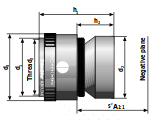
\includegraphics[width=\textwidth]{makro-symmar-hm.png}
\end{figure}


\end{document}
